\section{Quickstart}\label{quickstart}

The Cloudmesh Compute Cluster service allows you to execute analytical,
computational workflows which run programs on remote compute resources.
We specify not only a list of tasks to be executed, but the tasks can
also have dependencies between each other expressed through a direct,
cyclic graph. Currently, we have predefined task types that can execute
shell scripts, Python programs, and Python notebooks, all of which can
be executed on local or remote compute resources.

In Figure 1 we depict a simple example workflow to be executed where
each task is executed sequentially. The status of the execution can be
displayed as table or as graph. In Figure 1, we showcase how the graph
changes its appearance over time.

\begin{longtable}[]{@{}
  >{\raggedright\arraybackslash}p{(\columnwidth - 8\tabcolsep) * \real{0.2083}}
  >{\raggedright\arraybackslash}p{(\columnwidth - 8\tabcolsep) * \real{0.1944}}
  >{\raggedright\arraybackslash}p{(\columnwidth - 8\tabcolsep) * \real{0.1806}}
  >{\raggedright\arraybackslash}p{(\columnwidth - 8\tabcolsep) * \real{0.1944}}
  >{\raggedright\arraybackslash}p{(\columnwidth - 8\tabcolsep) * \real{0.1944}}@{}}
\toprule
\begin{minipage}[b]{\linewidth}\raggedright
Step 0
\end{minipage} & \begin{minipage}[b]{\linewidth}\raggedright
Step 0.5
\end{minipage} & \begin{minipage}[b]{\linewidth}\raggedright
Step 1
\end{minipage} & \begin{minipage}[b]{\linewidth}\raggedright
Step 2
\end{minipage} & \begin{minipage}[b]{\linewidth}\raggedright
Step 3
\end{minipage} \\
\midrule
\endhead
Definition & Running first task & Finished first task & Finished second
task & Completed workflow \\
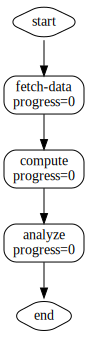
\includegraphics{images/workflow-example.svg} &
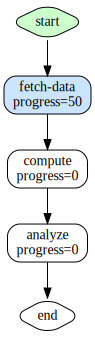
\includegraphics{images/workflow-example-1.5.svg} &
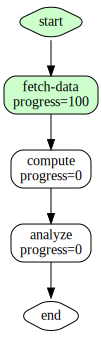
\includegraphics{images/workflow-example-2.svg} &
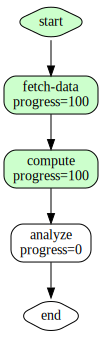
\includegraphics{images/workflow-example-3.svg} &
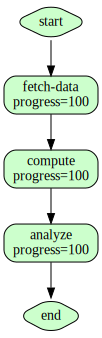
\includegraphics{images/workflow-example-5.svg} \\
\bottomrule
\end{longtable}

\textbf{Figure 1:} Execution and display graph of an example workflow
over time

We can specify such workflows in a YAML file making it very easy to
create and manage them. To get you started, we have developed a
quickstart example that you can enhance to get acquainted with the
system.

Once a workflow is specified, it can be executed a using one of our
interfaces. This includes a Python API and a command line interface
without a REST service. In addition we have, with the help of the Python
API, developed a REST service so that integration into other frameworks
can be facilitated through REST calls. The availability of the REST
service is important to access it from non Python frameworks, but also
allows the easy interaction through a Web-based Portal.

Let us demonstrate a number of selected features with the help of this
quickstart. We will only focus on using the REST service.

\subsection{Setup}\label{setup}

To start, the code is needed and we assume you are standing in the
cloudmesh-cc directory. Use the following commands

\begin{verbatim}
```bash
git clone https://github.com/cloudmesh/cloudmesh-cc.git
cd cloudmesh-cc
pip install -e .
```
\end{verbatim}

We also assume you start the service with

\begin{verbatim}
```bash
cms cc start --reload
```
\end{verbatim}

\subsection{Creating a simple example}\label{creating-a-simple-example}

First let us create a simple workflow example that we already have
included for you in our source code. We will use this workflow and copy
it into a temporary directory:

\begin{verbatim}
```bash
mkdir -p /tmp/workflow-example
cp tests/workflow-example/workflow-example.yaml /tmp/workflow-example
cp tests/workflow-example/*.sh /tmp/workflow-example
```
\end{verbatim}

We like you to inspect the example so you get an overview of how to
define a workflow that is located in
\href{https://github.com/cloudmesh/cloudmesh-cc/tree/main/tests/workflow-example}{GitHub}:
and is located in the folder \emph{tests/workflow-example/}

\begin{itemize}
\tightlist
\item
  \href{https://github.com/cloudmesh/cloudmesh-cc/blob/main/tests/workflow-example/workflow-example.yaml}{workflow-example.yaml}
\item
  \href{https://github.com/cloudmesh/cloudmesh-cc/blob/main/tests/workflow-example/fetch-data.sh}{fetch-data.sh}
\item
  \href{https://github.com/cloudmesh/cloudmesh-cc/blob/main/tests/workflow-example/compute.sh}{compute.sh}
\item
  \href{https://github.com/cloudmesh/cloudmesh-cc/blob/main/tests/workflow-example/analyze.sh}{analyze.sh}
\end{itemize}

Now we can test a selected number of ways on how to interact with the
service. We showcase here how to

\begin{itemize}
\item
  \begin{enumerate}
  \def\labelenumi{\Alph{enumi}.}
  \tightlist
  \item
    upload workflows as tar/xz file of a self containing directory, or
  \end{enumerate}
\item
  \begin{enumerate}
  \def\labelenumi{\Alph{enumi}.}
  \setcounter{enumi}{1}
  \tightlist
  \item
    upload all files in a directory recursively
  \end{enumerate}
\end{itemize}

\subsection{A. Upload and run a workflow embedded in an archive
file}\label{a.-upload-and-run-a-workflow-embedded-in-an-archive-file}

We can upload an archive file which contains all the workflow files,
including the yaml specification file and the scripts. Providing an
archive file such as a \texttt{.tar}, \texttt{.tar.gz}, or \texttt{.xz}.
may enable the workflow to be better suited towards portability and
simplicity, where one can share an archive file with another user. We
will choose here a tar file as example.

\subsubsection{Create tar archive file}\label{create-tar-archive-file}

Before uploading a \texttt{tar} archive file, we must first create it
using the previous example yaml and scripts that we copied.

\begin{verbatim}
```bash
tar -C /tmp/workflow-example -cf workflow-example.tar .
```
\end{verbatim}

\subsubsection{\texorpdfstring{Option 1: Upload via
\texttt{curl}}{Option 1: Upload via curl}}\label{option-1-upload-via-curl}

We can upload the archive file by using the \texttt{curl} terminal
command as follows:

\begin{verbatim}
```bash
curl -X 'POST' \
  'http://127.0.0.1:8000/workflow?archive=workflow-example.tar' \
  -H 'accept: application/json' \
  -d ''
```
\end{verbatim}

\subsubsection{\texorpdfstring{Option 2: Upload via
\texttt{/docs}}{Option 2: Upload via /docs}}\label{option-2-upload-via-docs}

As the service is using also an OpenAPI 2.0 specification the workflow
can also be uploaded implicitly through the specification GUI. Navigate
to \texttt{http://127.0.0.1:8000/docs} and use the POST Upload method.

\begin{figure}
\centering
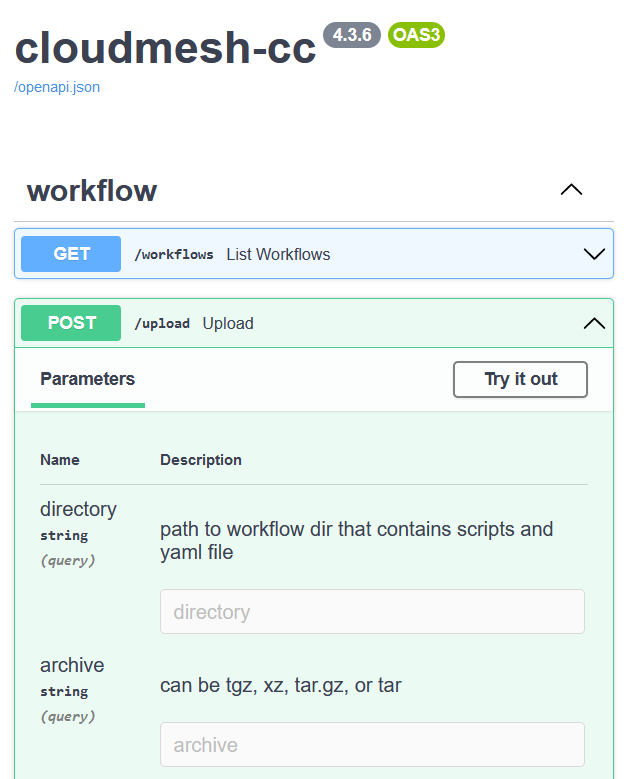
\includegraphics[width=1.1\columnwidth]{images/upload_api.png}
\caption{Browser API GUI for Cloudmesh Compute Cluster}
\end{figure}

Please click \texttt{Try\ it\ out} and then enter
\texttt{\textasciitilde{}/cm/cloudmesh-cc/workflow-example.tar} in the
\texttt{archive} field and then click Execute.

\subsubsection{Option 3: Upload via the Python
API}\label{option-3-upload-via-the-python-api}

As we use a REST service, we can also easily upload the workflow through
a Python enabled REST call. We will use Python requests to demonstrate
this upload feature.

\begin{Shaded}
\begin{Highlighting}[]
\ImportTok{import}\NormalTok{ requests}

\NormalTok{r }\OperatorTok{=}\NormalTok{ requests.post(}\StringTok{\textquotesingle{}http://127.0.0.1:8000/workflow?archive=workflow{-}example.tar\textquotesingle{}}\NormalTok{)}
\BuiltInTok{print}\NormalTok{(r)}
\BuiltInTok{print}\NormalTok{(r.text)}
\end{Highlighting}
\end{Shaded}

Printing \texttt{r} returns the response code from the API (a code of
200 indicates success). Printing \texttt{r.text} returns the message
from the API, such as a success or error message.

\subsubsection{Option 4: Upload with a third party REST
framework}\label{option-4-upload-with-a-third-party-rest-framework}

Naturally if you like to use a different REST API you can do so. You can
also use different programming languages and we leave it up to you to
choose the framework of your choice to interact with the REST service,
popular choices are JavaScript, Go, C/C++, matlab, and R, to name a few.

\subsection{B. Upload a dir that contains workflow
directory}\label{b.-upload-a-dir-that-contains-workflow-directory}

To increase flexibility and allow quick experiments, users can specify a
workflow directory which contains the yaml specification file and the
scripts. This way, pre-archival of the directory is not needed. The
program sets up the workflow by copying the necessary files from the
specified directory.

There are three different ways to upload the dir: via \texttt{curl} on
the command line, via the browser GUI, and via the Python API.

\subsubsection{\texorpdfstring{Option 1: Upload via
\texttt{curl}}{Option 1: Upload via curl}}\label{option-1-upload-via-curl-1}

A workflow can be uploaded easily with a curl command from the command
line. On the command line execute:

\begin{Shaded}
\begin{Highlighting}[]
\ExtensionTok{curl} \AttributeTok{{-}X} \StringTok{\textquotesingle{}POST\textquotesingle{}} \DataTypeTok{\textbackslash{}}
  \StringTok{\textquotesingle{}http://127.0.0.1:8000/workflow?directory=\textasciitilde{}/cm/cloudmesh{-}cc/tests/workflow{-}example\textquotesingle{}} \DataTypeTok{\textbackslash{}}
  \AttributeTok{{-}H} \StringTok{\textquotesingle{}accept: application/json\textquotesingle{}} \DataTypeTok{\textbackslash{}}
  \AttributeTok{{-}d} \StringTok{\textquotesingle{}\textquotesingle{}}
\end{Highlighting}
\end{Shaded}

\subsubsection{\texorpdfstring{Option 2: Upload via
\texttt{/docs}}{Option 2: Upload via /docs}}\label{option-2-upload-via-docs-1}

Also here one can upload the needed files with the OpenAPI specification
interface on the service. Navigate to
\texttt{http://127.0.0.1:8000/docs} and use the POST Upload method.

Click \texttt{Try\ it\ out} and then enter
\texttt{\textasciitilde{}/cm/cloudmesh-cc/tests/workflow-example} in the
directory field and then click Execute.

\subsubsection{Option 3: Upload via the Python
API}\label{option-3-upload-via-the-python-api-1}

Accessing the upload from the Pythin API is very easy. We will use
python requests to demonstrate the upload of the workflow.

\begin{Shaded}
\begin{Highlighting}[]
\ImportTok{import}\NormalTok{ requests}

\NormalTok{r }\OperatorTok{=}\NormalTok{ requests.post(}\StringTok{\textquotesingle{}http://127.0.0.1:8000/workflow?directory=\textasciitilde{}/cm/cloudmesh{-}cc/tests/workflow{-}example\textquotesingle{}}\NormalTok{)}
\BuiltInTok{print}\NormalTok{(r)}
\BuiltInTok{print}\NormalTok{(r.text)}
\end{Highlighting}
\end{Shaded}

Printing \texttt{r} returns the response code from the API (a code of
200 indicates success). Printing \texttt{r.text} returns the message
from the API, such as a success or error message.

\subsection{Parameters to the Upload a workflow with a REST
call}\label{parameters-to-the-upload-a-workflow-with-a-rest-call}

The upload REST URL can take different parameters, such as

\begin{itemize}
\tightlist
\item
  \texttt{?directory=name}
\item
  \texttt{?archive=name.tar.gz}
\item
  \texttt{?archive=name.tgz}
\item
  \texttt{?archive=name.xz}
\item
  \texttt{?yaml=name}
\end{itemize}

The semantic of the upload is specified through its parameter. Only one
of them can be used at a time.

The directory parameter indicates that the contents of a specified
directory will be transferred into a workflow.

The archive parameter indicates that an archive file, such as a
\texttt{tar} file, will be extracted and its contents will be
transferred into a workflow. Please note that the \texttt{archive} and
\texttt{directory} parameters can not be used in the same REST call.

The yaml parameter indicates that only a yaml file will be uploaded
without any corresponding scripts. Uploading a yaml file by itself
allows for a script specified by the yaml to be uploaded later. The yaml
can even work without scripts by using the \texttt{exec} specification
within the yaml.

\subsection{Run the workflow}\label{run-the-workflow}

To run, navigate to homepage at \texttt{http://127.0.0.1:8000/} and
click the workflow-example on the left side. Then click Run.
